\documentclass[10pt,letterpaper]{article}
\usepackage[margin=0.7in,headheight=14pt]{geometry}
\usepackage[T1]{fontenc}
\usepackage{lmodern,microtype,amsmath,amssymb,booktabs,tabularx,array}
\usepackage[dvipsnames]{xcolor}
\usepackage{tikz}
\usetikzlibrary{arrows.meta,positioning,shapes.geometric}
\usepackage{enumitem,fancyhdr,listings,hyperref}
\definecolor{ink}{HTML}{19334A}
\definecolor{accent}{HTML}{007E87}
\definecolor{pale}{HTML}{EEF5F7}
\hypersetup{colorlinks=true,linkcolor=accent,urlcolor=accent,pdftitle={Job Scheduler: Design and Validation},pdfsubject={COP 5536 Fall 2026 programming project}}
\pagestyle{fancy}\fancyhf{}
\fancyhead[L]{\small\textcolor{ink}{COP 5536 \; / \; Fall 2026}}
\fancyhead[R]{\small Job Scheduler}
\fancyfoot[L]{\footnotesize Design and validation report}
\fancyfoot[R]{\thepage}
\setlength{\parindent}{0pt}\setlength{\parskip}{5pt}
\setlist[itemize]{nosep,leftmargin=1.3em}
\setlist[enumerate]{nosep,leftmargin=1.5em}
\newcolumntype{Y}{>{\raggedright\arraybackslash}X}
\newcommand{\code}[1]{\texttt{#1}}
\newcommand{\sectiontitle}[2]{\section*{\textcolor{accent}{#1}\quad #2}}
\lstset{basicstyle=\ttfamily\footnotesize,backgroundcolor=\color{pale},frame=single,rulecolor=\color{pale},breaklines=true,columns=fullflexible,keepspaces=true,xleftmargin=5pt,xrightmargin=5pt,aboveskip=6pt,belowskip=6pt}
\begin{document}
{\LARGE\bfseries\color{ink} Job Scheduler}\par
{\large Design, Algorithms, and Validation}\par
\textcolor{accent}{Programming project technical report \;\textbullet\; November 2026}

\sectiontitle{01}{Program organization}
The simulator reads timestamped commands, manages a fixed execution capacity $k$, and writes deterministic results. Its two required data structures are implemented from scratch: an AVL tree indexes non-cancelled jobs by ID, and a binary max heap ranks waiting jobs. Java standard-library collections support running-job tracking, cancellation history, and execution history.

\begin{center}
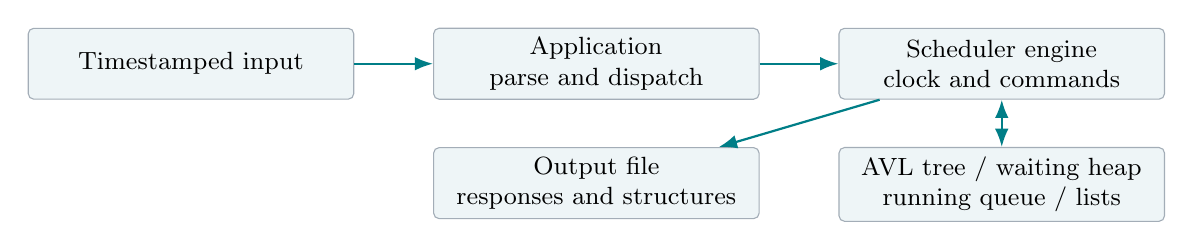
\begin{tikzpicture}[node distance=6mm and 10mm,>=Latex,
 box/.style={draw=ink!40,rounded corners=2pt,fill=pale,align=center,font=\small,minimum height=9mm,text width=39mm},
 arr/.style={->,thick,draw=accent}]
\node[box] (input) {Timestamped input};
\node[box,right=of input] (parser) {Application\\parse and dispatch};
\node[box,right=of parser] (engine) {Scheduler engine\\clock and commands};
\node[box,below=of engine] (data) {AVL tree / waiting heap\\running queue / lists};
\node[box,below=of parser] (out) {Output file\\responses and structures};
\draw[arr] (input)--(parser);\draw[arr] (parser)--(engine);
\draw[arr,<->] (engine)--(data);\draw[arr] (engine)--(out);
\end{tikzpicture}
\end{center}

\begin{tabularx}{\linewidth}{@{}lY@{}}\toprule
\textbf{Submission file} & \textbf{Responsibility}\\\midrule
\code{jobScheduler.java} & Default-package launcher for the required invocation.\\
\code{JobSchedulerApplication.java} & Reads capacity and commands; dispatches operations; writes the output file.\\
\code{SchedulerEngine.java} & Owns simulation time, capacity, job lifecycle, and output assembly.\\
\code{Job.java} & Stores ID, submission time, priority, estimate, delta, status, and execution timestamps.\\
\code{AvlTree.java} & Implements ID lookup, insertion, deletion, balancing, traversals, and counters.\\
\code{OutputFormat.java} & Centralizes required output labels, templates, and locale-independent formatting.\\
\code{AvlTreeStatistics.java} & Immutable record containing an AVL statistics snapshot.\\
\code{HeapStatistics.java} & Immutable record containing a waiting-heap statistics snapshot.\\
\code{WaitingMaxHeap.java} & Implements waiting-job ranking, indexed removal, priority repair, and policy rebuild.\\\bottomrule
\end{tabularx}

\textbf{Shared job identity.} Each accepted submission creates one \code{Job}. The AVL node and waiting heap reference that same object. Starting transfers the reference from the waiting heap into the running queue and execution history. Cancellation removes it from the AVL tree and waiting heap, then appends it to the cancellation list. This avoids divergent copies of status or timing fields.

\textbf{Record ownership.} The AVL tree retains WAITING, RUNNING, and COMPLETED jobs. Cancelled jobs remain in cancellation order in an \code{ArrayList}. Lookup searches the AVL tree first and then this list; cancelled IDs remain reserved against duplicate submission.

\textbf{Submission layout.} All nine source files, \code{Makefile}, \code{README.md}, and this PDF are at the archive root. The development scheduler class is named \code{JobScheduler}; packaging renames it to \code{SchedulerEngine} and removes package declarations from generated copies. This meets the flat-layout requirement and avoids a filename collision with \code{jobScheduler.java} on case-insensitive systems.

\newpage
\sectiontitle{02}{Data structures and scheduling algorithms}
\textbf{AVL tree.} A node stores a key, a shared job reference, left and right child links, and cached height. With $h(\varnothing)=0$ and $h(\text{leaf})=1$, the balance factor is
\[
  \operatorname{BF}(v)=h(v_L)-h(v_R),\qquad |\operatorname{BF}(v)|\leq 1.
\]
Insertion follows the BST path, then refreshes heights and rebalances while recursion returns. Deletion handles zero or one child directly; for two children, the inorder successor supplies both the replacement key and job reference. The successor is removed from the right subtree before rebalancing.

\begin{tabularx}{\linewidth}{@{}lYY@{}}\toprule
\textbf{Imbalance} & \textbf{Repair} & \textbf{Primitive counters}\\\midrule
Left--left & Right rotation & Right $+1$\\
Right--right & Left rotation & Left $+1$\\
Left--right & Left child rotates left; root rotates right & Left $+1$, right $+1$\\
Right--left & Right child rotates right; root rotates left & Right $+1$, left $+1$\\\bottomrule
\end{tabularx}

\textbf{Binary max heap.} An \code{ArrayList<Job>} holds the actual heap. For zero-based index $i$, the parent is $\lfloor(i-1)/2\rfloor$ and children are $2i+1$ and $2i+2$. An auxiliary \code{HashMap<Integer,Integer>} maps IDs to positions; it is an index, not a replacement heap. Every swap updates both positions.

The ``maximum'' is the job with the highest scheduling rank. Equivalently, choose the lexicographically smallest tuple below (the minus sign expresses descending priority mathematically; the implementation compares directly):
\[
\begin{aligned}
\text{PRIORITY:}&\quad(-\text{priority},\ \text{submission},\ \text{ID}),\\
\text{SHORT\_JOBS:}&\quad(\text{estimate},\ -\text{priority},\ \text{submission},\ \text{ID}).
\end{aligned}
\]
Insertion sifts upward. Extraction or cancellation replaces the removed entry with the last entry, then repairs upward or downward as needed. A successful priority update also repairs the existing entry. The first \code{SHORT\_JOBS} command changes the comparator and uses bottom-up heap construction; later submissions use the new mode. Repeated commands print the required acknowledgement but do not rebuild again.

\textbf{Time and capacity.} A standard \code{PriorityQueue<Job>} orders running jobs by completion time, then ID for deterministic ties. Before each command at $t$, all jobs with completion time $\leq t$ are marked COMPLETED. A \code{PROCESS\_NEXT} operation proceeds as follows:
\begin{enumerate}
\item If no job is waiting, emit \code{NO\_WAITING\_JOBS}.
\item If all $k$ slots are occupied, advance to the earliest completion and complete every job due at that instant.
\item Extract one waiting job, set its start time to the current clock, and record it in the running queue and execution history.
\end{enumerate}
\[
\text{actual}=\text{estimate}+\Delta,\qquad
\text{completion}=\text{start}+\text{actual}.
\]
\begin{center}
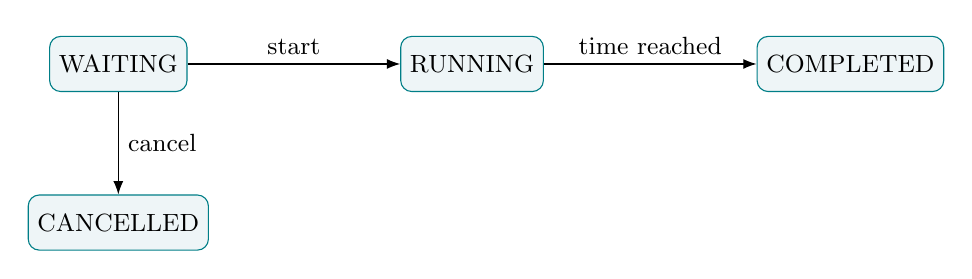
\begin{tikzpicture}[>=Latex,node distance=13mm and 27mm,every node/.style={font=\small},s/.style={draw=accent,rounded corners,fill=pale,minimum height=7mm}]
\node[s] (w) {WAITING};\node[s,right=of w] (r) {RUNNING};\node[s,right=of r] (f) {COMPLETED};
\node[s,below=of w] (c) {CANCELLED};
\draw[->] (w)--node[above]{start}(r);\draw[->] (r)--node[above]{time reached}(f);
\draw[->] (w)--node[right]{cancel}(c);
\end{tikzpicture}
\end{center}
Jobs are not preempted. Waiting jobs are not automatically started, and running jobs are not drained at end of input. SHORT\_JOBS uses estimated time only, not estimated time plus delta.

\newpage
\sectiontitle{03}{Complexity and output correctness}
Let $n$ be the current AVL record count, $w$ the waiting count, $r\leq k$ the running count, and $c$ the cancelled count. Define $L=O(\log(n+1)+c)$ for lookup including the possible cancellation-list scan. Hash-map access is expected $O(1)$; heap bounds below assume that expected access cost. Each command also processes any newly due completions: $q$ completions add $O(q\log(k+1))$.

\begin{tabularx}{\linewidth}{@{}l l Y@{}}\toprule
\textbf{Operation} & \textbf{Time, excluding due completions} & \textbf{Explanation}\\\midrule
AVL search/insert/delete & $O(\log(n+1))$ & Balanced search path and local rotations.\\
SUBMIT & $O(L+\log(w+1))$ & Duplicate lookup, tree insertion, heap insertion.\\
FIND & $O(L)$ & AVL lookup followed by cancellation scan.\\
CANCEL / UPDATE\_PRIORITY & $O(L+\log(w+1))$ & Locate job and repair heap; cancellation also deletes an AVL entry.\\
PROCESS\_NEXT & $O(\log(w+1)+\log(k+1))$ & Extract waiting job and insert running job; a capacity wait may complete up to $k$ jobs.\\
First SHORT\_JOBS & $O(w)$ expected & Bottom-up heap rebuild and index reconstruction.\\
JOB\_STATUS & $O(n+c)$ & Inorder traversal followed by cancellation list.\\\bottomrule
\end{tabularx}

The core job records and collection references occupy $O(N)$ space for $N$ accepted submissions. The application additionally buffers all input lines and output strings, so total memory includes their text size. The tree level renderer retains full positional NULL placeholders internally; its work can reach $O(2^h)$ for height $h$, even though trailing NULLs are omitted in the printed representation. This is a reporting cost rather than a search/update cost.

\textbf{Worked trace: supplied case 3.} At 55 ms the policy changes to SHORT\_JOBS. At 57 ms, waiting job 104 is cancelled. At 58 ms both slots are occupied, so the next start waits until job 102 completes at 60 ms. Job 105 has the shortest remaining estimate and starts at 60 ms. At 60 ms the next request again finds full capacity and waits until job 105 completes at 80 ms; job 106 then starts. Job 101 remains waiting.

\begin{minipage}[t]{0.47\linewidth}
\begin{lstlisting}
EXECUTION_ORDER
102 20 60
103 30 130
105 60 80
106 80 150
END_EXECUTION_ORDER
\end{lstlisting}
\end{minipage}\hfill
\begin{minipage}[t]{0.50\linewidth}
\begin{lstlisting}
TREE
LEVEL 0: [105]
LEVEL 1: [102]|[106]
LEVEL 2: [101]|[103]
END_TREE
MAX_HEAP: [(101,3,60)]
\end{lstlisting}
\end{minipage}

\textbf{Formatting contract.} Command responses use the exact required labels and punctuation, without explanatory \code{Input:} or \code{Output:} prefixes. FIND fields are ordered as submitted, started, actual\_time, completed, and status. Unknown timing fields print lowercase \code{null}. JOB STATUS prints non-cancelled records by increasing ID, followed by cancelled records in cancellation order.

Final sections appear as execution order, tree, inorder traversal, heap, tree statistics, and heap statistics, matching the supplied cases. Tree levels use bracketed IDs, \code{|} separators and uppercase \code{NULL}. Heap tuples are \code{(ID,priority,estimate)} in actual array order. Counters distinguish extraction from cancellation removal, and double rotations count as two primitive rotations. Empty structures still emit their opening/closing labels and empty lists where applicable.

\newpage
\sectiontitle{04}{Validation, build, and dependencies}
\textbf{Acceptance evidence.} The development test suite contains 17 fixed input files and 30 seeded random scenarios. Each random scenario has 150 commands, for 4,500 generated commands in addition to the fixed cases. The random scenarios use large timestamp gaps to satisfy the input guarantee that later commands do not precede a capacity-induced clock advance; the fixed cases separately exercise capacity waits and simultaneous completions.

\begin{tabularx}{\linewidth}{@{}l Y@{}}\toprule
\textbf{Test group} & \textbf{Evidence and assertions}\\\midrule
3 instructor DOCX cases & Compare complete output with supplied answers after whitespace normalization, including exact tree shape, heap array and statistics.\\
2 PDF examples & Exercise priority selection and shortest-estimate selection, including capacity waits.\\
12 additional fixed cases & Empty queues; duplicate/missing jobs; cancellation errors and order; priority and short-job ties; priority repair; simultaneous completions; large timestamps; LL, RR, LR, RL rotations; deletion rebalancing.\\
30 seeded model comparisons & Compare messages, statuses and execution history with an independent list-based scheduler, avoiding the production AVL, heap and running priority queue.\\
Structural assertions & Check BST ordering, AVL balance and height, inorder membership, heap membership and parent rank, and mutation counts. Minimal rotation cases also check exact root/children and primitive rotation counts.\\
Isolated submission build & Extract the flat ZIP into a temporary directory, compile it independently, supply the 17 fixed inputs from the development tests, and compare their output.\\\bottomrule
\end{tabularx}

The three instructor-provided expected files are the external oracle for exact structural examples. Other expected files are regression snapshots checked against the independent behavioral model; they are not additional instructor answers. Random tests validate structural invariants, not a unique AVL shape or exact rotation count for every possible input. These checks provide correctness evidence for the covered inputs rather than an exhaustive proof.

\textbf{Static analysis.} SpotBugs 4.10.4 and strict compiler checks (\code{-Xlint:all -Werror}) run as development checks. A possible output-path null dereference was fixed, and regression tests check null rejection before heap mutation, empty extraction, and malformed command syntax. The only SpotBugs exclusion permits the assignment-required lowercase launcher name; null-pointer rules remain enabled.

\textbf{Build and execution.} The application uses JDK 17 language/API compatibility via \code{javac --release 17}. No external Java libraries, Gradle invocation, or network access is needed when a compatible JDK is already installed.
\begin{lstlisting}
make
java jobScheduler input_file
# Optional Makefile run target:
make run INPUT=path/to/input.txt
\end{lstlisting}
The grading environment supplies Java. The Makefile invokes \code{javac} and \code{java} directly; it does not check for or install Java. All application imports belong to the Java standard library. No additional JAR files, dependency managers, downloads, Python, Docker, or LaTeX are needed to build or run the submission. Python is used only for development tests and packaging; LaTeX is used only to produce this report.

\textbf{Output location.} An input such as \code{cases/input.txt} produces \code{cases/input\_output\_file.txt}. Results go to that file; build diagnostics remain outside it. Submission verification has run locally on macOS with JDK 27 targeting release 17. An Ubuntu execution has not been directly verified.

\textbf{Scope and assumptions.} Inputs follow the assignment's capacity, timestamp, unique-job intent, and positive-actual-duration guarantees. The parser is designed for that command grammar, not recovery from arbitrary malformed input. IDs and priorities use Java \code{int}; timing fields use \code{long}, with arithmetic assumed to remain within its range.

\textbf{Report production.} This PDF is compiled from \code{report/Report.tex} using LaTeX. The development project retains the source and build script; the submission includes only the compiled report. The program organization and formatting requirements are taken from the course's \emph{ADS+Project.pdf}; the three complete reference cases are from \emph{TestCases.docx}.
\end{document}
